\section{The defense}\label{sec:defense}
Keeping in mind our theoretical model, we determine the key elements that make these
attacks possible.

We propose a defense, \textit{context hiding}, that mitigates a class of
practical compression side-channel attacks such as CRIME, TIME, BREACH, Rupture,
and HEIST. The full plaintext recovery these attacks perform is no longer
possible when our defense is applied.

\subsection{Hardness of defending}
First of all, observe that there is a trivial method of defense, and that is
disabling compression completely. To see why this successfully defends against
an adversary in the adaptive reflection game, observe that when $f$ outputs a
constant length, if Com is the identity function, then the attacker cannot
obtain any more information than the simulator provided that Enc is a secure
encryption scheme.

We now point the attention of the reader to the fact that defending against an
adversary by modifying $f$ is hard in general. We note that $f$ is required to
be polynomially reversible, meaning it must contain enough information to
recover $s$. Because Com, as a compression function, must be able to decrease
the length of various plaintexts, it can output plaintexts of different
lengths, and hence dependent on the string $s$. Therefore, if Com is
adversarial, it can easily leak information through the encryption function Enc
by using its output length. As such, any attempt to generally defend against
all compression functions Com is necessarily futile.

However, given the fact that it is theoretically difficult to define a generic
defense should not discourage us from pursuing a practical defense that applies
in practice given the specific compression functions which are in use in the
real-world. As mentioned previously, such compression functions are difficult
to deal with in an analytical manner, as they are technically involved. We
therefore do not provide a formal proof that our defense method is secure.
However, we give a series of arguments for why we believe this is the case
based on our previously developed theory.

\subsection{Attack elements from a defense perspective}
The basic problem that needs be solved is the compression detectability of
the predicate $Q$ under this class of attacks. In order to eliminate detectability,
it should be made impossible for any pair of reflections $\overbar{r}$ to detect
$Q$ under the compression function $\textrm{Com}$ and the rendering function $f$. In order to
achieve this there exist two options - either change the compression or the
rendering function.

The next step is determining what the form of the needed changes is. We
therefore consider the notions that make detectability possible.
These notions are compression idealness and interdependence. The first is part
of the composition of $\textrm{Com}$ and $f$ whereas the second is part of $f$. That
said, removing either of these notions from the functions will strip the
adversary the ability to detect $Q$.

The first choice is forcing the compression function to act non-ideally in the
cases of secrets. Proposed defenses like disabling compression for annotated
secrets, or for the whole response, serve this exact idea.

The second choice is removing the interdependece between reflections and
secrets. In order to achieve that we need to decorrelate the probability of each
secret from the reflection. A method that uses this option is secret masking,
described in section \ref{subsec:masking}. Context hiding also builds on this
option and is described in the following sections.

\subsection{Context hiding properties}

Context hiding is built on the premise of separating secrets in a per-origin
manner in order to avoid cross-compression. In order to achieve this we define
what constitutes an origin and what properties same-origin secrets share. This
section describes the key components of the defense and the code implementation.

\subsubsection{Origins}
An origin is a uniquely identifiable party that generates content. A party can
be either a physical entity, like a user, or an application that provides a
service. It is important to properly identify the party that generated, or could
have generated, a piece of content. The definition of origins should reflect the
ability to generate all content that is assigned to each origin.

\subsubsection{Same-origin secrets}
Defining origins is the first step to identifying same-origin secrets. Secrets
are content pieces that are assinged to origins. Secrets that are assigned to an
origin should have been generated by the party that this origin identifies.
Also the origin's party has access to all content in this origin. This results
in a secret $a$ being insecure for all other secrets belonging in $a$'s origin.

\subsection{Context hiding functionality}
Our defense method proposes disabling cross-compression by applying a simple
substitution cipher derived from a random permutation of the plaintext alphabet.

Firstly, we identify the origins based on the output $m$ of rendering function
$f$ and store them in array $origins$. Each secret $s_i$ in $m$ is then
separated based on its origin. Each origin is uniquely identified by an integer
in range $[0, |origins|-1)$.

Secondly, we identify the alphabet for each origin. An origin's alphabet
consists of all possible characters that a secret of this origin may contain.
For each origin, we generate a random permutation of the origin's alphabet and
store it in the array $permutations$. The first element in the $permutations$
array corresponds to the first origin in the $origins$ array and so forth.

In order to secure a secret $s$ we apply a hiding function. The hiding function
\textit{hide} takes two arguments, the secret $s$ and the permutation $p$ of the
secret's origin. It applies the substitution cipher on each character in $s$ and
returns the permuted secret $s'$. The substitution cipher is implemented in the
function $Permute_p(c)$, which finds the index $i$ of character $c$ in the sorted
permutation $p$ and replaces it with the $i$-th character in $p$.

\begin{lstlisting}[texcl,mathescape,basicstyle=\small]
def hide($s, p$):
    $s' = ''$
    for $ch \in s$:
        $s' = s' || Permute_p(ch)$
    return $s'$
\end{lstlisting}

The protected secret $s'$ is annotated by the special characters
$\beta_{start}^i$, $\beta_{end}^i$ that mark the start and the end of any
substring that needs to be unpermuted.

The output $m'$ that is produced after hiding all secrets includes the
permutation array $permutations$, so that applying the reverse permutation on
all secrets is possible.

The permuted secrets in $m'$ can be retrieved using the special annotation
characters $\beta_{start}^i$ and $\beta_{end}^i$ that are unique per origin.

The initial secret $s$ can be retrieved from the protected secret $s'$
using the \textit{unhide} function. This function takes secret $s'$ and
permutation $p$ of the secret's origin and applies the reverse permutation on
$s'$, returning the unpermuted secret $s$.

\begin{lstlisting}[texcl,mathescape,basicstyle=\small]
def unhide($s', p$):
    $s = ''$
    for $ch \in s'$:
        $s = s || Unpermute_p(ch)$
    return $s$
\end{lstlisting}

In this defense, note that we have generalized the fact that there is no single
secret that needs to be protected, which was a simplification of our
theoretical model. In practice, for the developer, the reflection $r$ and the
secret $s$ are two secrets that have different origins.

Given the fact that $s$ and $r$ are permuted every time an oracle call is made
makes it difficult for an adversary controlling $r$ to learn information about
$s$.

Our defense is implemented in the application layer and is opt-in. We choose to
update the rendering function $f$ instead of the compression function
$\textrm{Com}$ as it is easier that way for web developers to incorporate it in
their applications. Our proposal requires no changes in the underlying
compression algorithms in the web server such as Apache's mod\_deflate, which
would require a huge engineering effort. Instead, our proposed defense requires
only modifications in the web application layer, which can be relatively easily
incorporated in existing applications.

\section{CTX: Mitigating BREACH with Context Hiding }\label{sec:ctx}

\subsection{Implementation}
Our contributions include the development of the CTX defense. CTX is an
implementation of the context hiding method described in the previous section
for HTML web pages.

It is up to the application developer to decide which portions of the response
are sensitive and must be protected as secrets. Sensitive data does not only
include high-value secrets such as passwords and CSRF tokens, but also user data
that the developer wishes to keep private. Some examples are the bodies of email
messages in Gmail, the chat messages received or sent to a friend on Facebook,
the contents of documents and spreadsheets in Google Docs and the list of online
friends on Facebook or Google Hangouts, as they contain all the important
contacts of the victim. Practically any piece of information which is only
accessible when logged in is potentially a secret and should be CTX protected.
On the other hand, some data do not typically need compression-security
protection, e.g. static HTML portions that are accessible on a website even when
logged out.

The minimum amount of origins is one origin for the entire response, in which
case CTX is not protecting any part of the plaintext, and the maximum is one
origin per character. The latter would result in the best possible security
under CTX, although compression would be effectively disabled - possibly resulting
in poor performance. This is the case with defenses such as secret masking.

Different-origin secrets are then forced to compress separately, i.e. not
cross-compress. However, compression is achieved within each context. The
default origin alphabet is ASCII characters (0 - 128). In order to randomly
permute the secret alphabet, we use the Fisher-Yates shuffle
algorithm \cite{fisher1938statistical}.

Secrets are then permuted by the server using the generated permutation of the
corresponding origin prior to TLS encryption and network transmission. Upon
arrival on the client side, the inverse permutation is applied to decode the
secret. The same permutation is applied to all secrets of the same origin. That
way, better compression is achieved intra-origin.

Each time the server issues an HTTPS response, new per-origin permutations are
generated. Compression side-channel attacks in general rely on the assumption that we can
perform multiple requests to the target website while the transmitted secret
remains the same. Since new alphabet permutations are generated per HTTPS
response, the statistical analysis performed by Rupture is no longer feasible.

\subsection{Experimental results}\label{subsec:ctx_experiments}

We have conducted several experiments to evaluate the performance of web
services protected by CTX. The results of these experiments are overwhelmingly
positive.

The CTX parameters that affect performance are basically 3: the number of
origins, the total response size in bytes, and the amount of
secrets in the response. Each parameter affects the performance differently and
will be examined thoroughly in the following sections. Our experiments focused
on each parameter separately, so the results reflect the performace under each
one independently.

In all our tests we use an HTML web page where the secrets are strings of
English literature. The tests measure the performance penalty in terms of size
overhead in the compressed response HTML. The penalty in execution time is
considered insignificant and not included when less than 10ms.

However, it should be noted that our tests are particularly strict. A typical
website response consists mainly of HTML code or libraries that usually need not
be protected. In this case, the amount of secrets in the response would not
exceed 1\% of the total response, in which case the CTX overhead as shown by our
experiments is acceptable. For example, Facebook and Gmail, which offer web
pages that are ~600KB typically need only protect approximately 0.5\% of the
response.

The first parameter, the number of origins, mainly affects the compression
performance of the secrets. The more origins are used the bigger the response,
both compressed and uncompressed, will be. This is expected, given the fact that
secrets from different origins do not cross-compress.

Our experiment covered a 650KB web page, which consists of 1\% secrets and 99\%
static data. The secrets are distributed in origins that range from 1 to 50, so
the length of a secret per origin is reduced as origins increase and the total
amount of secrets and static data remains the same. We consider 50 origins a
reasonable choice since a typical response contains data generated by multiple
users and web services.

    \begin{figure}[thpb]
        \centering
            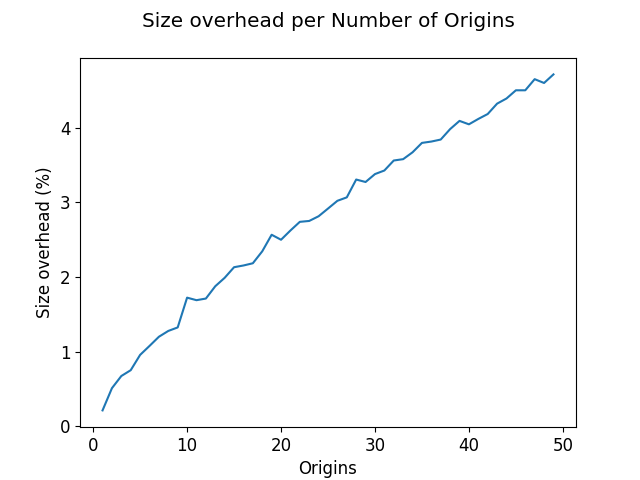
\includegraphics[width=0.48\textwidth]{experiments/origins.png}
        \caption{Origins}
        \label{fig:origin_ctx}
    \end{figure}

As Figure \ref{fig:origin_ctx} shows, the size overhead when 1 origin is used is less than 0.5\%
and about 4.7\% when 50 origins are used. This means that the compressed
response when CTX is used is expected to be 1.47x the unprotected compressed
response when 50 origins are used.

The second parameter, the total response size in bytes, affects the impact of
CTX on the compressed response.

In this case, we use 50 origins and consider 1\% of the total response to be
secret, equally distributed in all origins. The total response ranges from a
13KB to a 650KB web page.

Our experiments show that the increase in bytes that CTX adds is not
proportional to the increase of the total response size. This results in a
significant response size increase for small web pages, which becomes less
observable as the web page grows larger.

    \begin{figure}[thpb]
        \centering
            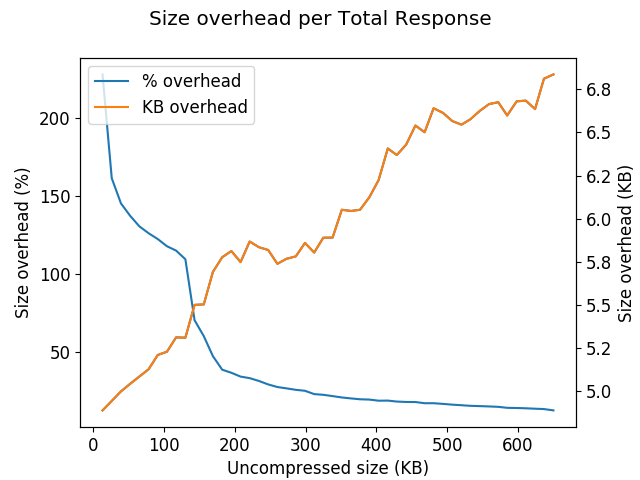
\includegraphics[width=0.48\textwidth]{experiments/total_response.png}
        \caption{Total response}
        \label{fig:total_response_ctx}
    \end{figure}

Figure \ref{fig:total_response_ctx} depicts the results of this experiment. A 13KB web page suffers a 5KB
CTX overhead, which corresponds to a 228\% increase in compressed response. On the
other hand, CTX will add only 7KB of compressed data for a 650KB web page, which
results in a 12\% increase. Disabling compression entirely would add overhead
that ranges from 500\% to 1000\% for the tested web pages.

The third parameter is the total amount of secrets in the response. In our
example we use a 650KB web page with 50 CTX origins. The secrets range from 1\%
up to 50\% of the web page, the rest being static data, and are evenly
distributed across origins.

    \begin{figure}[thpb]
        \centering
            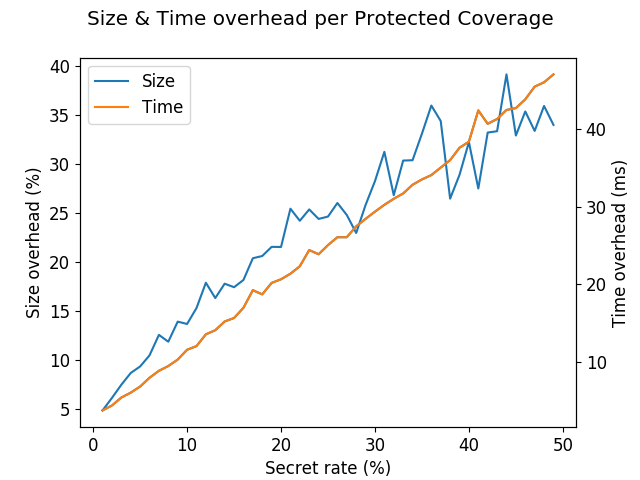
\includegraphics[width=0.48\textwidth]{experiments/response_secrets.png}
        \caption{Response secrets}
        \label{fig:response_secrets_ctx}
    \end{figure}

Figure \ref{fig:response_secrets_ctx} shows the results in this case. We find that protecting 1\% of the
tested web page results in less than 5\% size overhead, whereas protecting 50\% of
the page results in 35\%. This test also showed a noteworthy time increase in
execution time, where for 10\% secrets in the web page CTX adds 10ms of
execution time, while for 50\% it adds 47ms.

In comparison, disabling compression would again result in 976.8\% load overhead
and a network transmittion time overhead that, depending on the client's and the
server's network, may be several seconds.


